% This file was created with tikzplotlib v0.9.16.
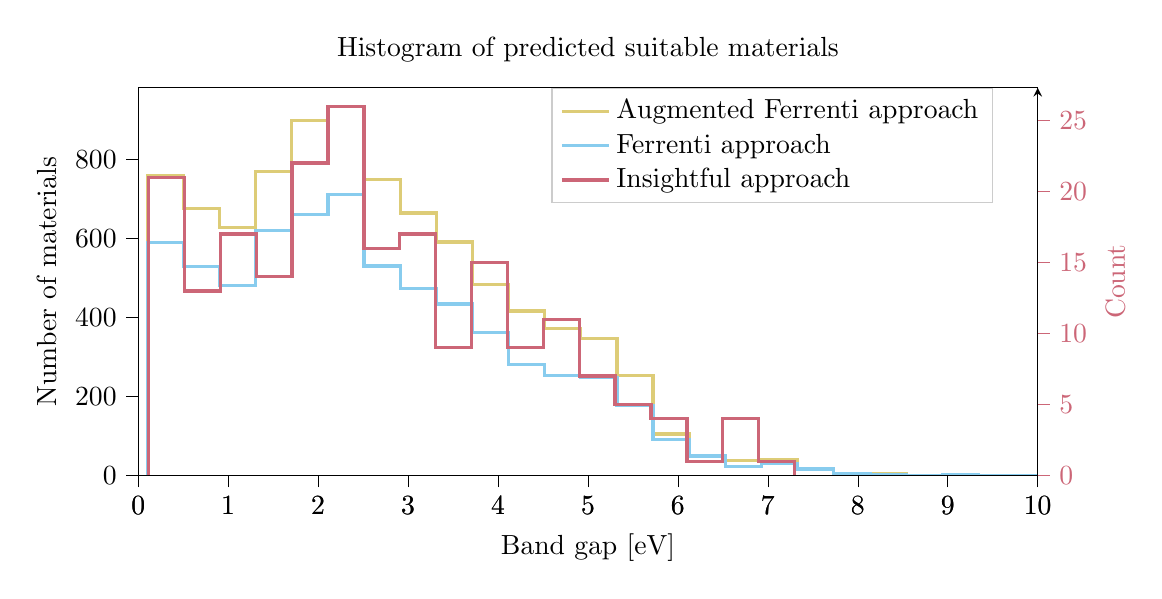
\begin{tikzpicture}

\definecolor{color0}{rgb}{0.866666666666667,0.8,0.466666666666667}
\definecolor{color1}{rgb}{0.533333333333333,0.8,0.933333333333333}
\definecolor{color2}{rgb}{0.8,0.4,0.466666666666667}

\begin{axis}[
height=2.5600388542963888in,
legend cell align={left},
legend style={fill opacity=0.8, draw opacity=1, text opacity=1, draw=white!80!black, at={(0.95,1)}},
tick align=outside,
tick pos=left,
title={Histogram of predicted suitable materials},
width=5.1200777085927776in,
x grid style={white!69.0196078431373!black},
xlabel={Band gap [eV]},
xmin=0, xmax=10,
xtick style={color=black},
y grid style={white!69.0196078431373!black},
ylabel={Number of materials},
ymin=0, ymax=980.7,
ytick style={color=black}
]
\path [draw=color0, very thick]
(axis cs:0.1003,0)
--(axis cs:0.1003,759)
--(axis cs:0.502006818181818,759)
--(axis cs:0.502006818181818,675)
--(axis cs:0.903713636363636,675)
--(axis cs:0.903713636363636,628)
--(axis cs:1.30542045454545,628)
--(axis cs:1.30542045454545,769)
--(axis cs:1.70712727272727,769)
--(axis cs:1.70712727272727,898)
--(axis cs:2.10883409090909,898)
--(axis cs:2.10883409090909,934)
--(axis cs:2.51054090909091,934)
--(axis cs:2.51054090909091,748)
--(axis cs:2.91224772727273,748)
--(axis cs:2.91224772727273,664)
--(axis cs:3.31395454545454,664)
--(axis cs:3.31395454545454,591)
--(axis cs:3.71566136363636,591)
--(axis cs:3.71566136363636,483)
--(axis cs:4.11736818181818,483)
--(axis cs:4.11736818181818,416)
--(axis cs:4.519075,416)
--(axis cs:4.519075,371)
--(axis cs:4.92078181818182,371)
--(axis cs:4.92078181818182,347)
--(axis cs:5.32248863636364,347)
--(axis cs:5.32248863636364,253)
--(axis cs:5.72419545454545,253)
--(axis cs:5.72419545454545,105)
--(axis cs:6.12590227272727,105)
--(axis cs:6.12590227272727,49)
--(axis cs:6.52760909090909,49)
--(axis cs:6.52760909090909,38)
--(axis cs:6.92931590909091,38)
--(axis cs:6.92931590909091,40)
--(axis cs:7.33102272727273,40)
--(axis cs:7.33102272727273,16)
--(axis cs:7.73272954545454,16)
--(axis cs:7.73272954545454,3)
--(axis cs:8.13443636363636,3)
--(axis cs:8.13443636363636,4)
--(axis cs:8.53614318181818,4)
--(axis cs:8.53614318181818,0)
--(axis cs:8.93785,0)
--(axis cs:8.93785,1)
--(axis cs:9.33955681818182,1)
--(axis cs:9.33955681818182,0)
--(axis cs:9.74126363636364,0)
--(axis cs:9.74126363636364,0)
--(axis cs:10.1429704545455,0)
--(axis cs:10.1429704545455,0)
--(axis cs:10.5446772727273,0)
--(axis cs:10.5446772727273,0)
--(axis cs:10.9463840909091,0)
--(axis cs:10.9463840909091,0)
--(axis cs:11.3480909090909,0)
--(axis cs:11.3480909090909,0)
--(axis cs:11.7497977272727,0)
--(axis cs:11.7497977272727,0)
--(axis cs:12.1515045454545,0)
--(axis cs:12.1515045454545,0)
--(axis cs:12.5532113636364,0)
--(axis cs:12.5532113636364,0)
--(axis cs:12.9549181818182,0)
--(axis cs:12.9549181818182,0)
--(axis cs:13.356625,0)
--(axis cs:13.356625,0)
--(axis cs:13.7583318181818,0)
--(axis cs:13.7583318181818,0)
--(axis cs:14.1600386363636,0)
--(axis cs:14.1600386363636,0)
--(axis cs:14.5617454545455,0)
--(axis cs:14.5617454545455,0)
--(axis cs:14.9634522727273,0)
--(axis cs:14.9634522727273,0)
--(axis cs:15.3651590909091,0)
--(axis cs:15.3651590909091,0)
--(axis cs:15.7668659090909,0)
--(axis cs:15.7668659090909,0)
--(axis cs:16.1685727272727,0)
--(axis cs:16.1685727272727,0)
--(axis cs:16.5702795454545,0)
--(axis cs:16.5702795454545,0)
--(axis cs:16.9719863636364,0)
--(axis cs:16.9719863636364,0)
--(axis cs:17.3736931818182,0)
--(axis cs:17.3736931818182,1)
--(axis cs:17.7754,1)
--(axis cs:17.7754,0);
\addlegendimage{line legend, draw=color0, very thick}
\addlegendentry{Augmented Ferrenti approach}

\path [draw=color1, very thick]
(axis cs:0.1003,0)
--(axis cs:0.1003,589)
--(axis cs:0.502006818181818,589)
--(axis cs:0.502006818181818,528)
--(axis cs:0.903713636363636,528)
--(axis cs:0.903713636363636,480)
--(axis cs:1.30542045454545,480)
--(axis cs:1.30542045454545,619)
--(axis cs:1.70712727272727,619)
--(axis cs:1.70712727272727,660)
--(axis cs:2.10883409090909,660)
--(axis cs:2.10883409090909,711)
--(axis cs:2.51054090909091,711)
--(axis cs:2.51054090909091,530)
--(axis cs:2.91224772727273,530)
--(axis cs:2.91224772727273,473)
--(axis cs:3.31395454545454,473)
--(axis cs:3.31395454545454,434)
--(axis cs:3.71566136363636,434)
--(axis cs:3.71566136363636,361)
--(axis cs:4.11736818181818,361)
--(axis cs:4.11736818181818,281)
--(axis cs:4.519075,281)
--(axis cs:4.519075,252)
--(axis cs:4.92078181818182,252)
--(axis cs:4.92078181818182,247)
--(axis cs:5.32248863636364,247)
--(axis cs:5.32248863636364,177)
--(axis cs:5.72419545454545,177)
--(axis cs:5.72419545454545,90)
--(axis cs:6.12590227272727,90)
--(axis cs:6.12590227272727,49)
--(axis cs:6.52760909090909,49)
--(axis cs:6.52760909090909,23)
--(axis cs:6.92931590909091,23)
--(axis cs:6.92931590909091,30)
--(axis cs:7.33102272727273,30)
--(axis cs:7.33102272727273,16)
--(axis cs:7.73272954545454,16)
--(axis cs:7.73272954545454,5)
--(axis cs:8.13443636363636,5)
--(axis cs:8.13443636363636,3)
--(axis cs:8.53614318181818,3)
--(axis cs:8.53614318181818,0)
--(axis cs:8.93785,0)
--(axis cs:8.93785,1)
--(axis cs:9.33955681818182,1)
--(axis cs:9.33955681818182,0)
--(axis cs:9.74126363636364,0)
--(axis cs:9.74126363636364,0)
--(axis cs:10.1429704545455,0)
--(axis cs:10.1429704545455,0)
--(axis cs:10.5446772727273,0)
--(axis cs:10.5446772727273,0)
--(axis cs:10.9463840909091,0)
--(axis cs:10.9463840909091,0)
--(axis cs:11.3480909090909,0)
--(axis cs:11.3480909090909,0)
--(axis cs:11.7497977272727,0)
--(axis cs:11.7497977272727,0)
--(axis cs:12.1515045454545,0)
--(axis cs:12.1515045454545,0)
--(axis cs:12.5532113636364,0)
--(axis cs:12.5532113636364,0)
--(axis cs:12.9549181818182,0)
--(axis cs:12.9549181818182,0)
--(axis cs:13.356625,0)
--(axis cs:13.356625,0)
--(axis cs:13.7583318181818,0)
--(axis cs:13.7583318181818,0)
--(axis cs:14.1600386363636,0)
--(axis cs:14.1600386363636,0)
--(axis cs:14.5617454545455,0)
--(axis cs:14.5617454545455,0)
--(axis cs:14.9634522727273,0)
--(axis cs:14.9634522727273,0)
--(axis cs:15.3651590909091,0)
--(axis cs:15.3651590909091,0)
--(axis cs:15.7668659090909,0)
--(axis cs:15.7668659090909,0)
--(axis cs:16.1685727272727,0)
--(axis cs:16.1685727272727,0)
--(axis cs:16.5702795454545,0)
--(axis cs:16.5702795454545,0)
--(axis cs:16.9719863636364,0)
--(axis cs:16.9719863636364,0)
--(axis cs:17.3736931818182,0)
--(axis cs:17.3736931818182,1)
--(axis cs:17.7754,1)
--(axis cs:17.7754,0);
\addlegendimage{line legend, draw=color1, very thick}
\addlegendentry{Ferrenti approach}

\addlegendimage{line legend, draw=color2, very thick}
\addlegendentry{Insightful approach}
\end{axis}

\begin{axis}[
axis y line=right,
height=2.5600388542963888in,
tick align=outside,
width=5.1200777085927776in,
x grid style={white!69.0196078431373!black},
xmin=0, xmax=10,
xtick pos=left,
xtick style={color=black},
y grid style={white!69.0196078431373!black},
ylabel=\textcolor{color2}{Count},
ymin=0, ymax=27.3,
ytick pos=right,
ytick style={color=color2},
yticklabel style={anchor=west, color=color2}
]
\path [draw=color2, very thick]
(axis cs:0.1157,0)
--(axis cs:0.1157,21)
--(axis cs:0.514638888888889,21)
--(axis cs:0.514638888888889,13)
--(axis cs:0.913577777777778,13)
--(axis cs:0.913577777777778,17)
--(axis cs:1.31251666666667,17)
--(axis cs:1.31251666666667,14)
--(axis cs:1.71145555555556,14)
--(axis cs:1.71145555555556,22)
--(axis cs:2.11039444444444,22)
--(axis cs:2.11039444444444,26)
--(axis cs:2.50933333333333,26)
--(axis cs:2.50933333333333,16)
--(axis cs:2.90827222222222,16)
--(axis cs:2.90827222222222,17)
--(axis cs:3.30721111111111,17)
--(axis cs:3.30721111111111,9)
--(axis cs:3.70615,9)
--(axis cs:3.70615,15)
--(axis cs:4.10508888888889,15)
--(axis cs:4.10508888888889,9)
--(axis cs:4.50402777777778,9)
--(axis cs:4.50402777777778,11)
--(axis cs:4.90296666666667,11)
--(axis cs:4.90296666666667,7)
--(axis cs:5.30190555555555,7)
--(axis cs:5.30190555555555,5)
--(axis cs:5.70084444444444,5)
--(axis cs:5.70084444444444,4)
--(axis cs:6.09978333333333,4)
--(axis cs:6.09978333333333,1)
--(axis cs:6.49872222222222,1)
--(axis cs:6.49872222222222,4)
--(axis cs:6.89766111111111,4)
--(axis cs:6.89766111111111,1)
--(axis cs:7.2966,1)
--(axis cs:7.2966,0);
\end{axis}

\end{tikzpicture}
